\documentclass[useAMS,usenatbib]{mn2e}
\usepackage{myaasmacros}
\usepackage{graphicx}
\usepackage{ulem}
\usepackage{amsmath}
\usepackage{multirow}


% Some definitions of things I always use here:
\newcommand\bcite[1]{\citeauthor{#1} \citeyear{#1}}


\title[Alignment of Light and Mass in Lensing Galaxies]{Alignment of Light and Mass in Lensing Galaxies}

\author[Bruderer]{Claudio Bruderer$^{1}$\thanks{E-mail: claudio.bruderer@phys.ethz.ch}, J. I. Read$^{1,2}$, P. Saha$^{3}$, J. Coles$^{4}$\\
$^{1}$Institute for Astronomy, Department of Physics, ETH Z\"urich, Wolfgang-Pauli-Strasse 27, CH-8093 Z\"urich, Switzerland\\
$^{2}$Department of Physics, University of Surrey, Guildford, GU2 7XH, UK\\
$^{3}$Institute for Theoretical Physics, University of Z\"urich, Winterthurerstrasse 190, 8057 Z\"urich, Switzerland\\
$^{4}$Department of Biology and Health, Versailles Saint-Quentin-en-Yvelines University, France
}

\begin{document}

\maketitle

\begin{abstract}
\end{abstract}

\begin{keywords}
Gravitational lensing: strong --- galaxies: structure
\end{keywords}


\section{Introduction}\label{sec:introduction}
\textbf{Content:}
\begin{itemize}
\item Understand galaxy structure
\item Relevant to e.g. weak lensing (Intrinsic alignments) and alternative gravity theories
\item Strong lensing reacts purely due to total mass distribution $\rightarrow$ Can disentangle light and mass
\item Free-form modelling technique, less model bias
\end{itemize}


\section{Data}\label{sec:data}
\textbf{Content:}
\begin{itemize}
\item Describe data set (why this data set, special features of galaxies (environment: y/n/unknonwn, elliptical/disk))
\end{itemize}

\begin{table*}
  \begin{center}
    \begin{tabular}
      ...
    \end{tabular}
    \caption[width=\linewidth]{Table with lens properties}
    \label{tab:lensproperties}
  \end{center}
\end{table*}

\begin{table*}
  \begin{center}
    \begin{tabular}
      ...
    \end{tabular}
    \caption[width=\linewidth]{Table with lens properties relevant for modelling (point masses, positions, time delays)}
    \label{tab:lensmodelling}
  \end{center}
\end{table*}


\section{Method}\label{sec:method}
\textbf{Content:}
\begin{itemize}
\item Describe GLASS
\item Describe shape measure and link it with Coles, Read and Saha 2014
\end{itemize}

\section{Results}\label{sec:results}
\textbf{Content:}
\begin{itemize}
\item Describe special features in reconstructed lenses
\item Show the wedges money plot
\item Discuss the results, especially:
\item 1. Dark matter halos seem quite round, stars not necessarily
\item 2. Dark matter halos are consistently more elliptical than stars
\item 3. Rather elliptical dark matter halos are more aligned, otherwise not really a clear trend
\item 4. There does not seem to be a trend of lenses being misaligned because of shear
\end{itemize}

\begin{figure*}
  \centering
  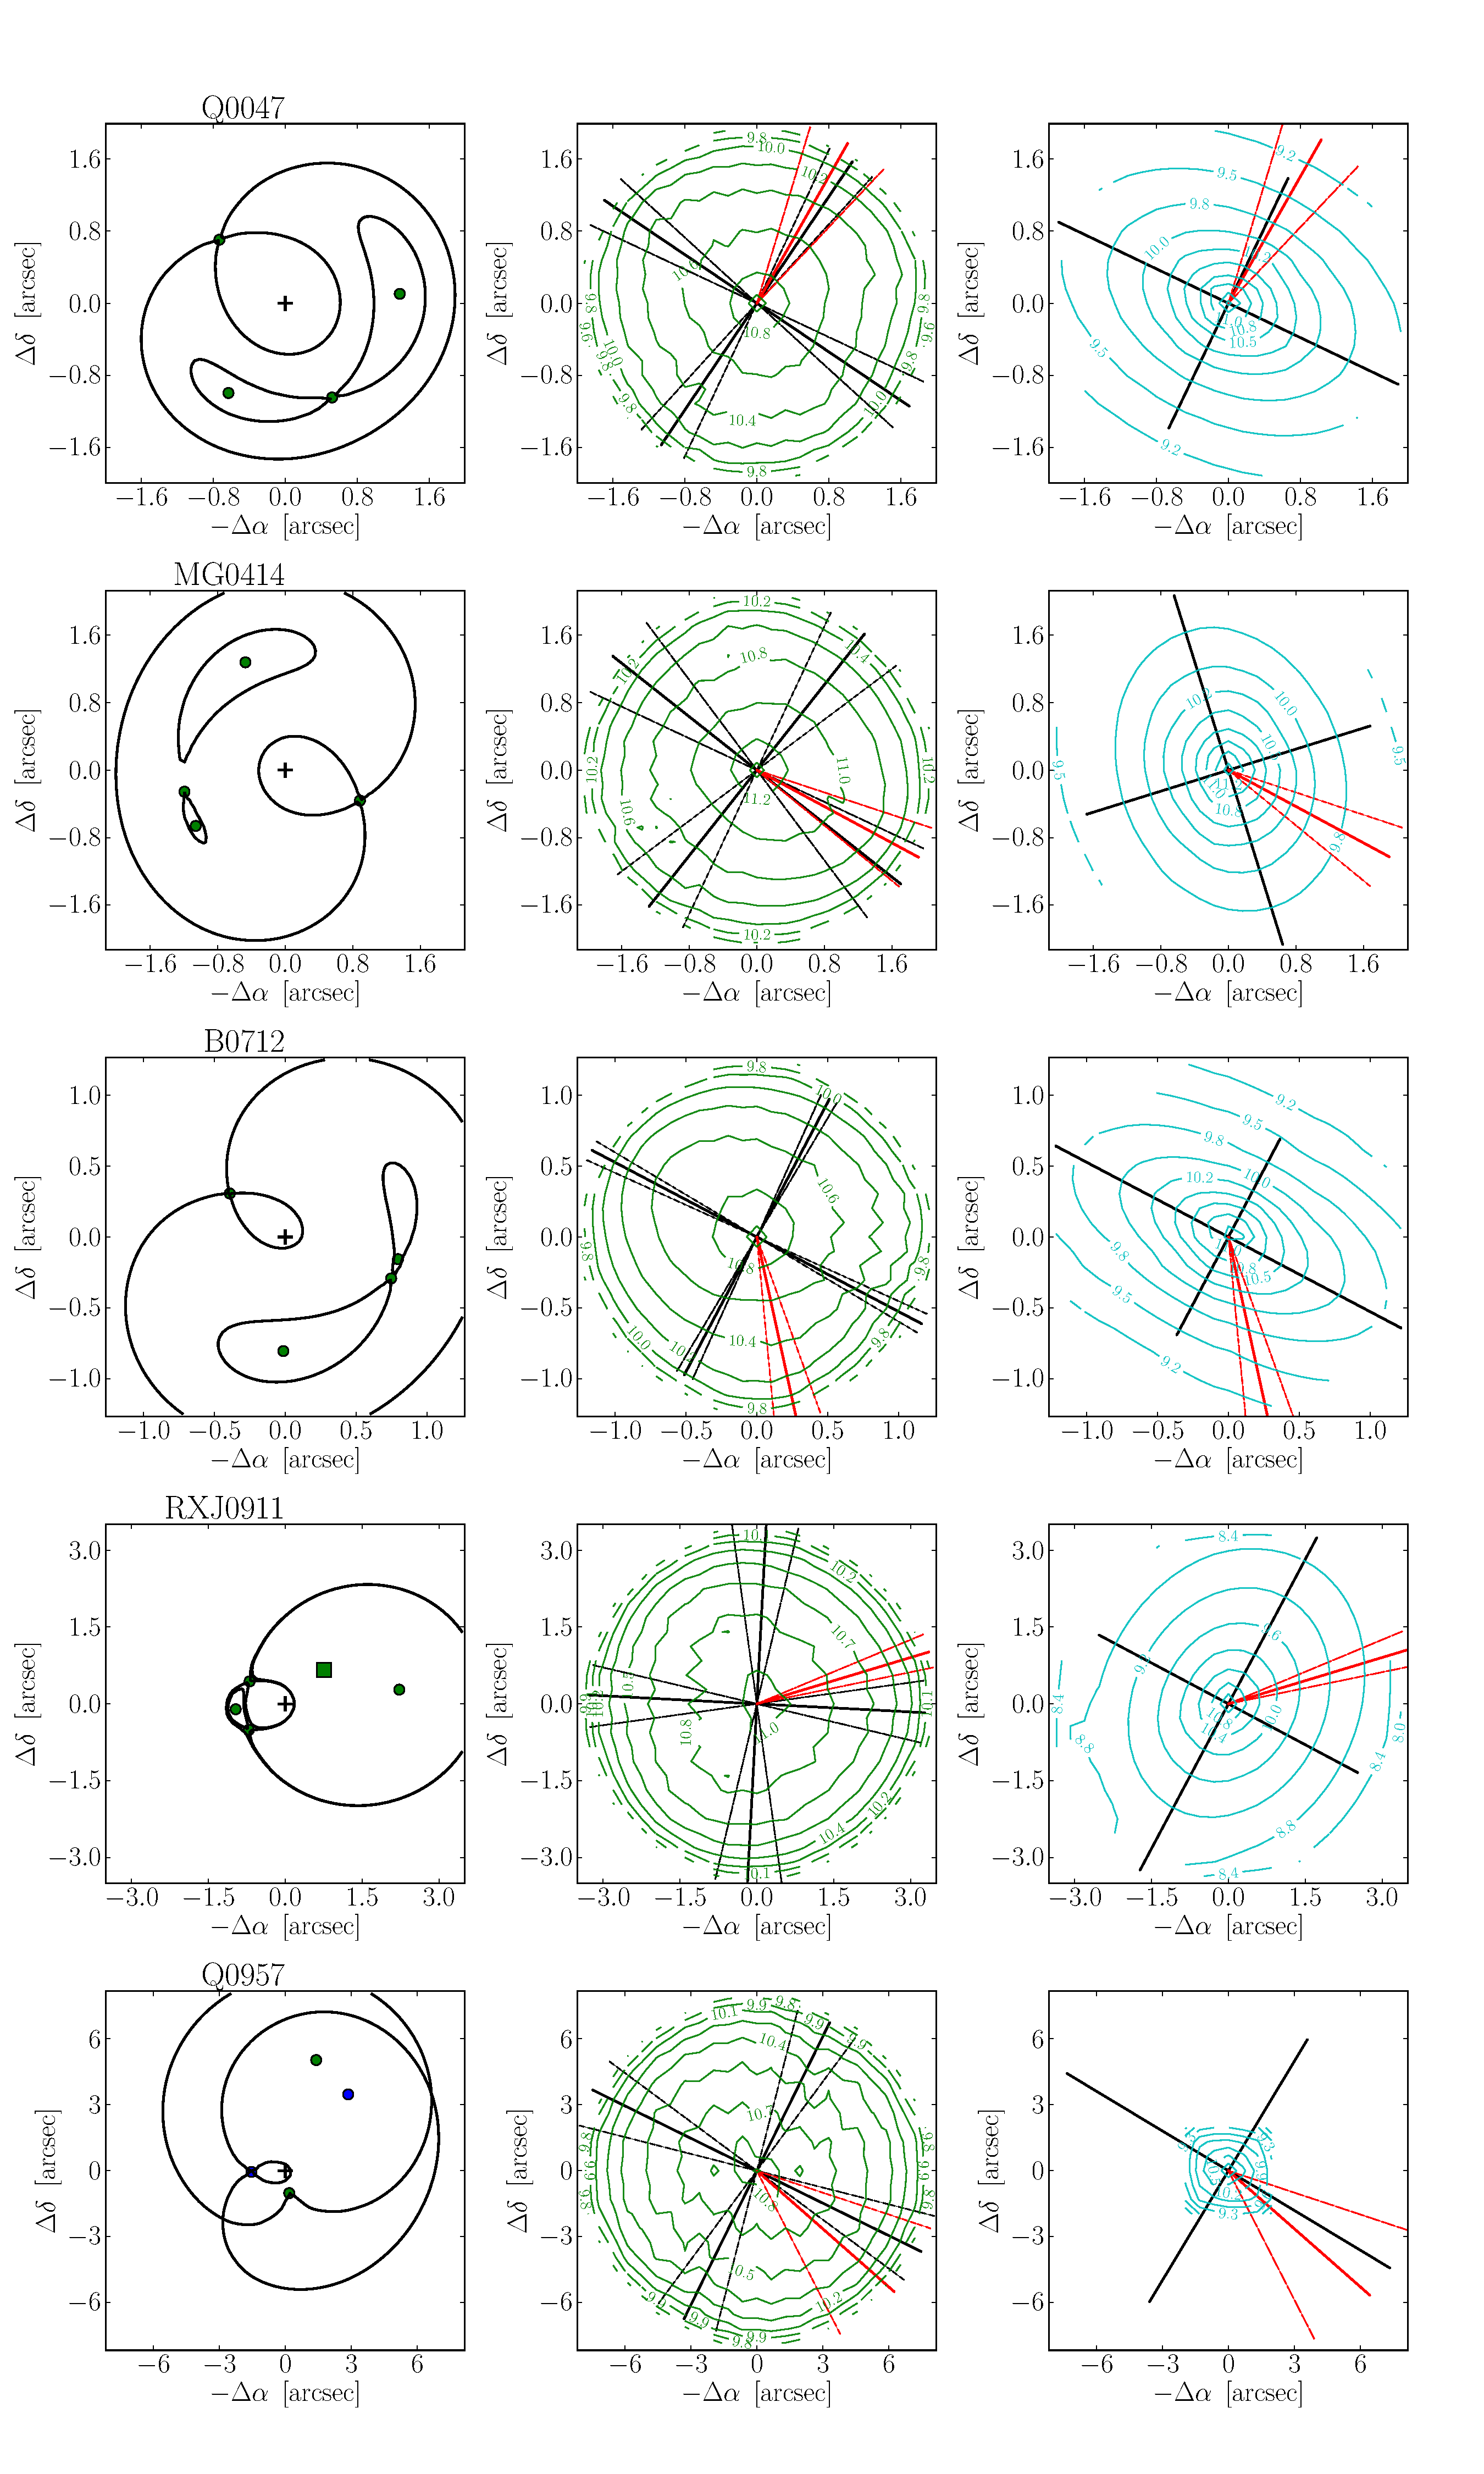
\includegraphics[width=.65\linewidth]{Figures/AllLenses21.pdf}
  \caption[width=.65\linewidth]{}
  \label{fig:lensreconstruction1}
\end{figure*}

\begin{figure*}
  \centering
  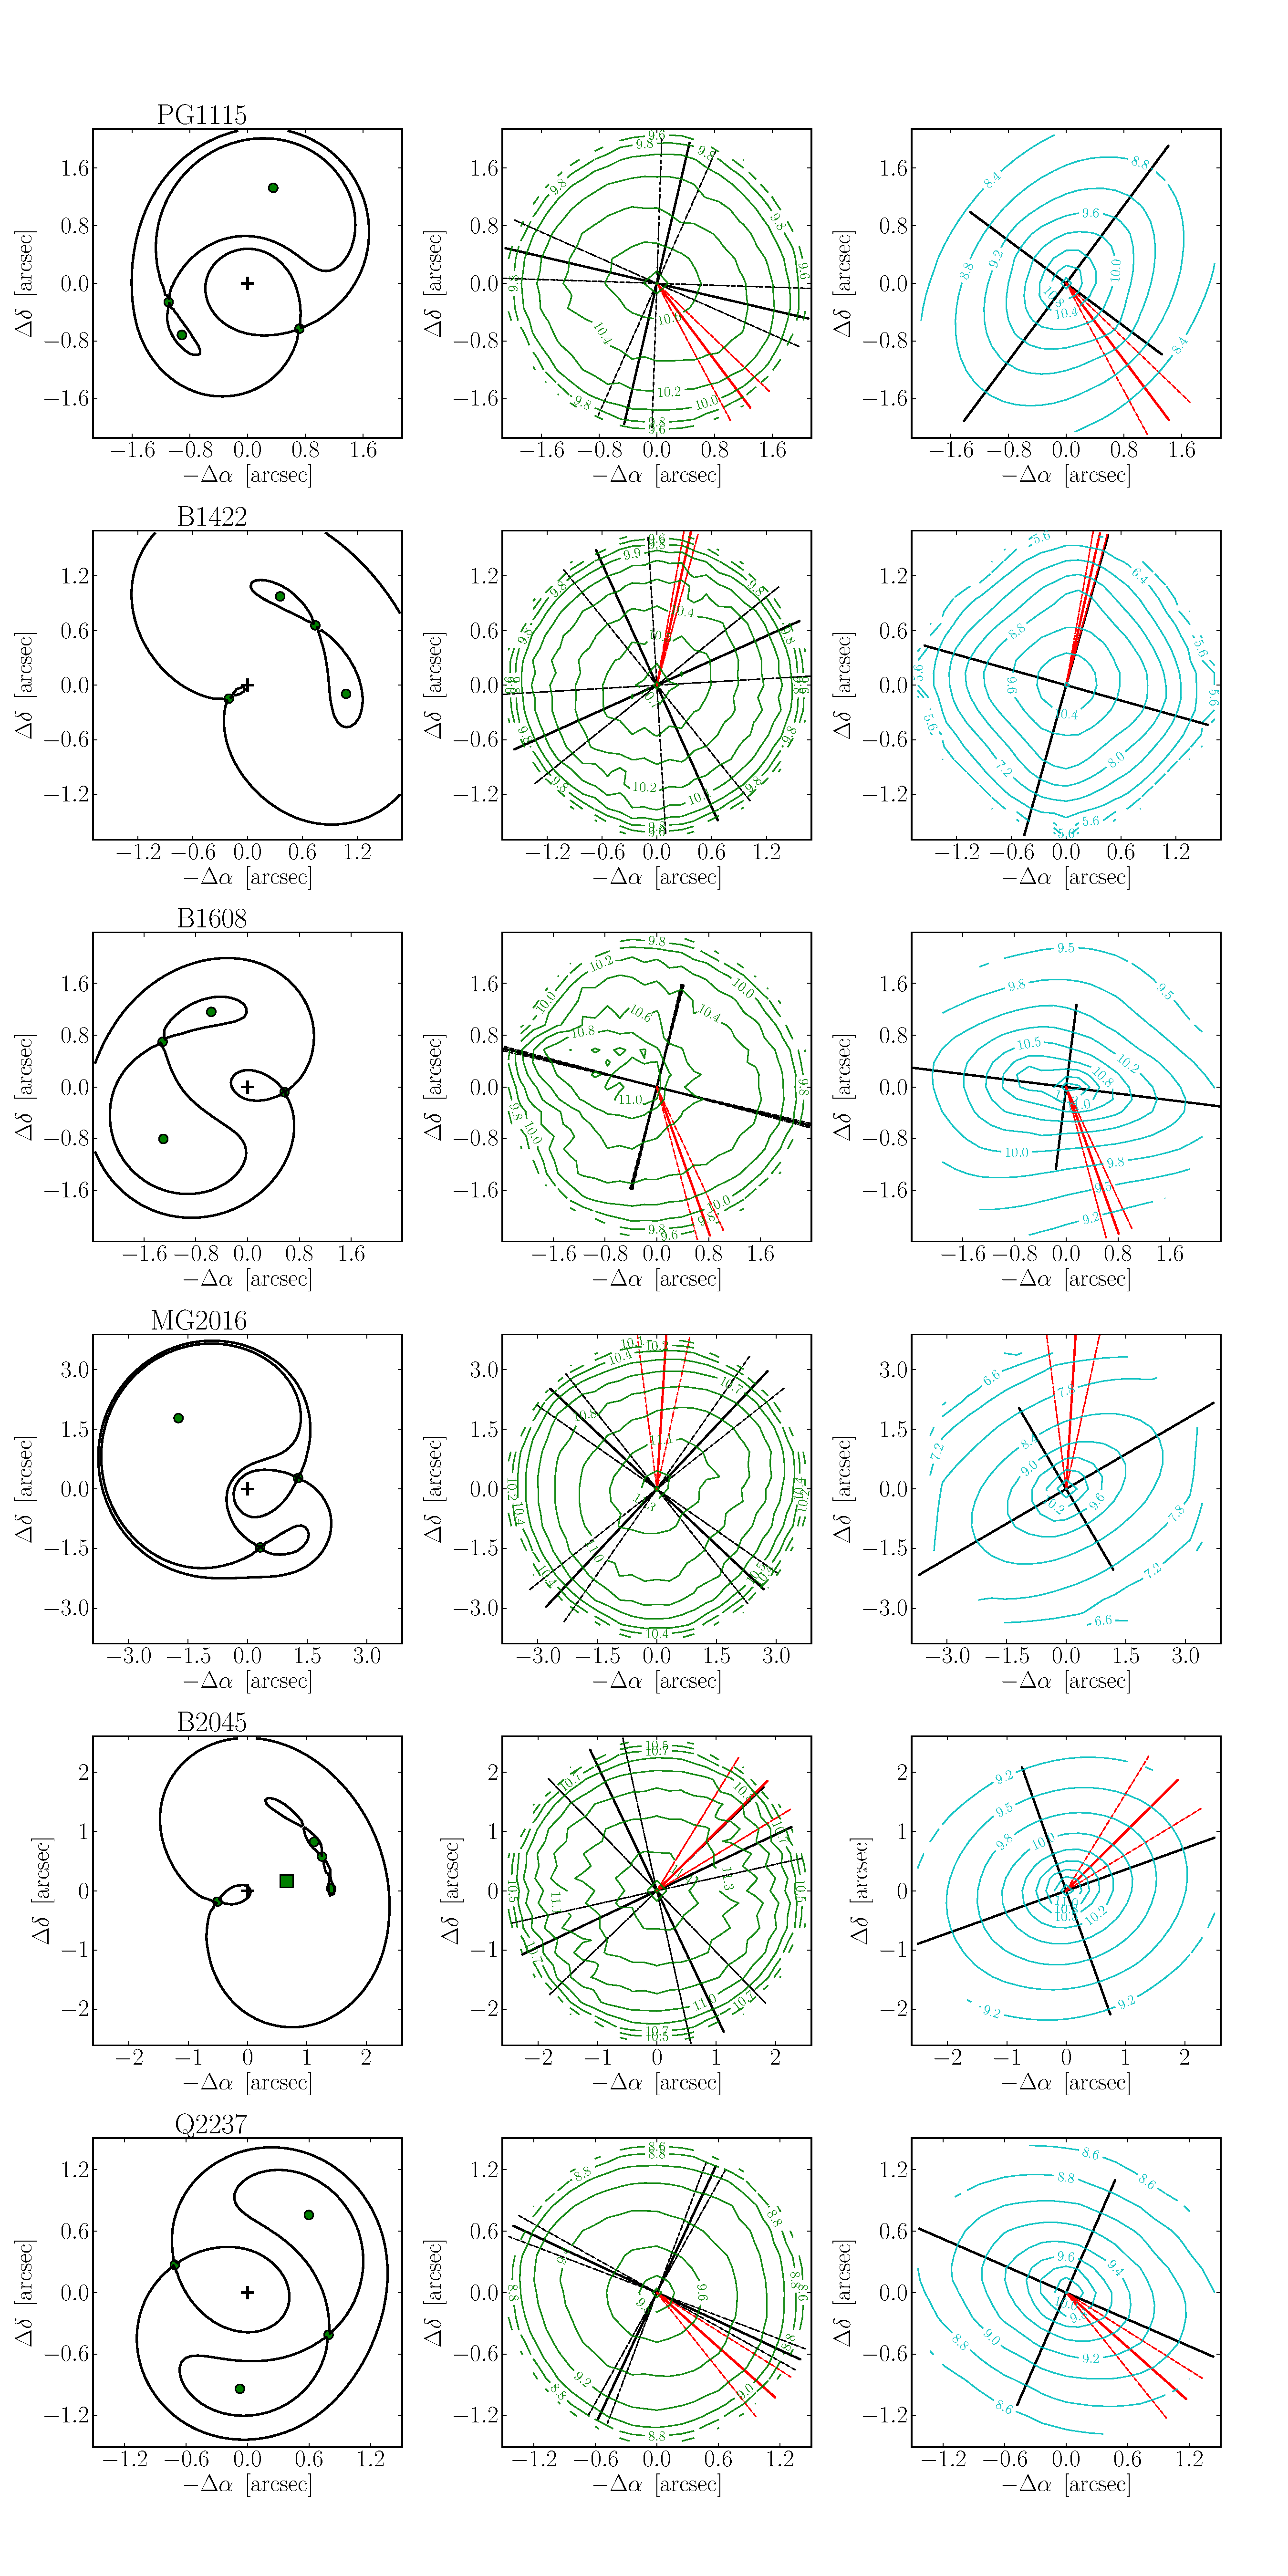
\includegraphics[width=.65\linewidth]{Figures/AllLenses22.pdf}
  \caption[width=.65\linewidth]{}
  \label{fig:lensreconstruction2}
\end{figure*}

\begin{figure*}
  \centering
  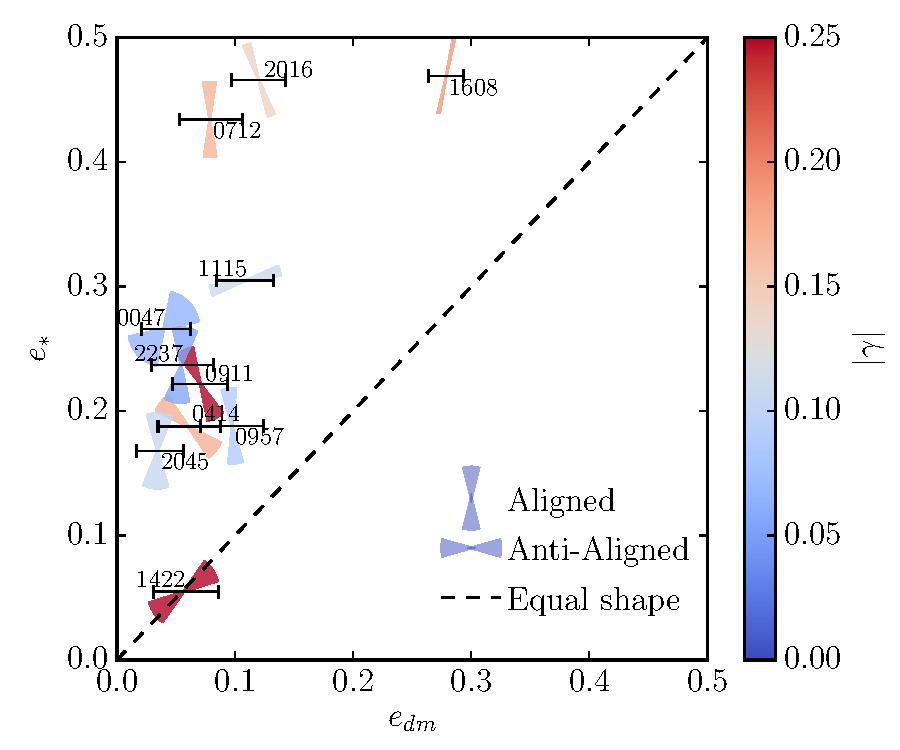
\includegraphics[width=.65\linewidth]{Figures/wedges_shears.pdf}
  \caption[width=.65\linewidth]{}
  \label{fig:wedges}
\end{figure*}

\section{Conclusion}\label{sec:conclusion}
...


\section{Acknowledgements}\label{sec:acknowledgements}
Acknowledge Dominik Leier, ...

JIR would like to acknowledge support from SNF grant PP00P2\_128540/1.

\bibliographystyle{mn2e}
\bibliography{paper}

%\clearpage
% \appendix
% \section{Reconstructed Lenses}\label{sec:reconstructions}

\end{document}